% docs/latex/ef-impact.tex
\documentclass{standalone}
\usepackage{tikz}
\usetikzlibrary{arrows.meta,backgrounds}

\begin{document}
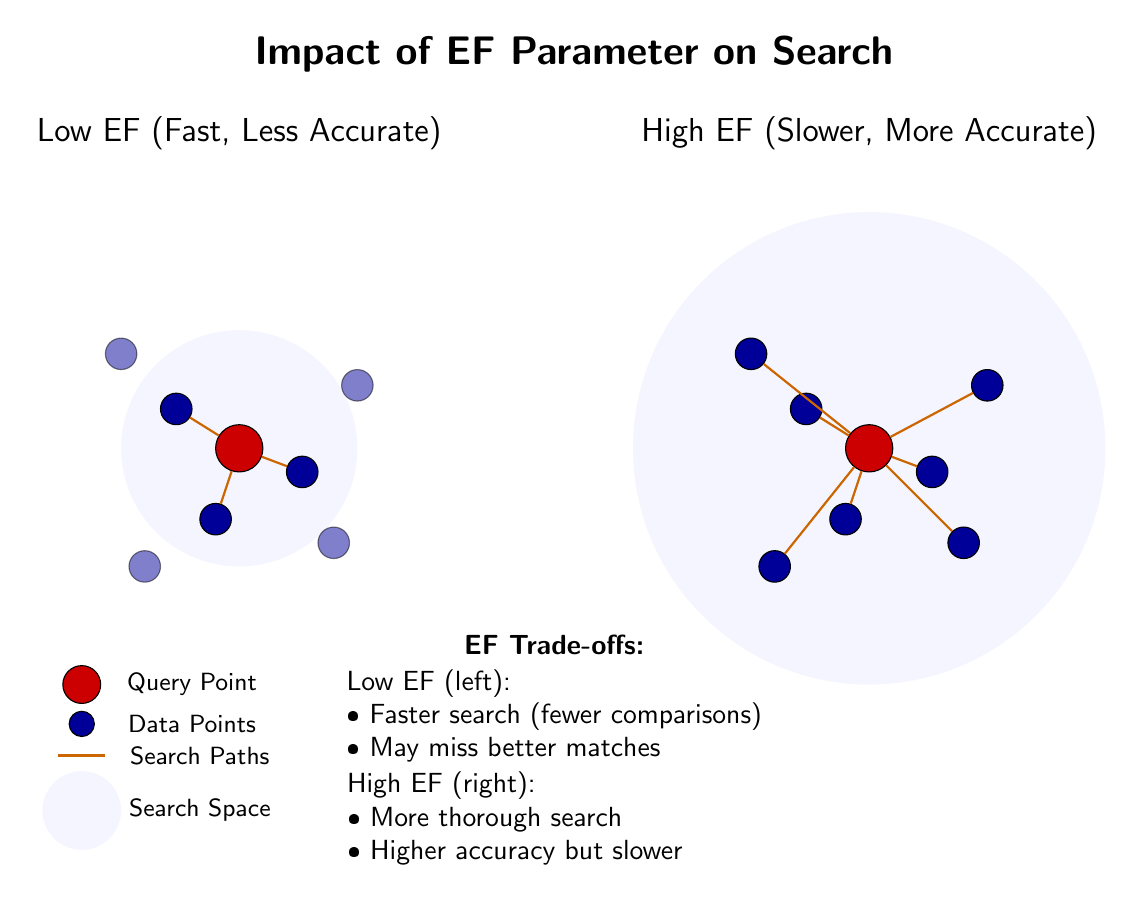
\begin{tikzpicture}[
    node/.style={circle, draw, fill=#1, minimum size=0.4cm},
    query node/.style={node=red!80!black, minimum size=0.6cm},
    data node/.style={node=blue!60!black},
    search path/.style={-, thick, orange!80!black},
    search space/.style={circle, fill=blue!20, opacity=0.2}
]

% Title
\node[font=\Large\sffamily\bfseries] at (0.25,6) {Impact of EF Parameter on Search};

% Section Labels
\node[font=\sffamily\large] at (-4,5) {Low EF (Fast, Less Accurate)};
\node[font=\sffamily\large] at (4,5) {High EF (Slower, More Accurate)};

% Low EF Search Space
\begin{scope}[shift={(-4,1)}]
    % Search space circle
    \node[search space, minimum size=3cm] at (0,0) {};
    
    % Query point
    \node[query node] (Q1) at (0,0) {};
    
    % Nearby nodes (visited)
    \node[data node] (L1) at (-0.8,0.5) {};
    \node[data node] (L2) at (0.8,-0.3) {};
    \node[data node] (L3) at (-0.3,-0.9) {};
    
    % Search paths
    \draw[search path] (Q1) -- (L1);
    \draw[search path] (Q1) -- (L2);
    \draw[search path] (Q1) -- (L3);
    
    % Outside nodes (not visited)
    \node[data node, opacity=0.5] at (-1.5,1.2) {};
    \node[data node, opacity=0.5] at (1.5,0.8) {};
    \node[data node, opacity=0.5] at (1.2,-1.2) {};
    \node[data node, opacity=0.5] at (-1.2,-1.5) {};
\end{scope}

% High EF Search Space
\begin{scope}[shift={(4,1)}]
    % Search space circle
    \node[search space, minimum size=6cm] at (0,0) {};
    
    % Query point
    \node[query node] (Q2) at (0,0) {};
    
    % All nodes (visited)
    \node[data node] (H1) at (-0.8,0.5) {};
    \node[data node] (H2) at (0.8,-0.3) {};
    \node[data node] (H3) at (-0.3,-0.9) {};
    \node[data node] (H4) at (-1.5,1.2) {};
    \node[data node] (H5) at (1.5,0.8) {};
    \node[data node] (H6) at (1.2,-1.2) {};
    \node[data node] (H7) at (-1.2,-1.5) {};
    
    % Search paths
    \foreach \n in {H1,H2,H3,H4,H5,H6,H7} {
        \draw[search path] (Q2) -- (\n);
    }
\end{scope}

% Legend
\begin{scope}[shift={(-6,-3)}]
    \node[query node, scale=0.8] at (0,1) {};
    \node[font=\small\sffamily] at (1.4,1) {Query Point};
    
    \node[data node, scale=0.8] at (0,0.5) {};
    \node[font=\small\sffamily] at (1.4,0.5) {Data Points};
    
    \draw[search path] (-0.3,0.1) -- (0.3,0.1);
    \node[font=\small\sffamily] at (1.5,0.1) {Search Paths};
    
    \node[search space, minimum size=1cm] at (0,-0.6) {};
    \node[font=\small\sffamily] at (1.5,-0.6) {Search Space};
\end{scope}

% Performance Comparison
\begin{scope}[shift={(0,-3)}]
    \node[font=\sffamily\bfseries] at (0,1.5) {EF Trade-offs:};
    \node[font=\sffamily, align=left] at (0,0.6) {Low EF (left):\\
        • Faster search (fewer comparisons)\\
        • May miss better matches};
    \node[font=\sffamily, align=left] at (-0.5,-0.7) {High EF (right):\\
        • More thorough search\\
        • Higher accuracy but slower};
\end{scope}

\end{tikzpicture}
\end{document}